\documentclass{standalone}

\usepackage{tikz}
\usetikzlibrary{patterns,arrows,calc,decorations.pathmorphing,backgrounds, positioning,fit,petri,decorations.fractals,trees}
\usepackage{xfrac}
	
\begin{document}
	
	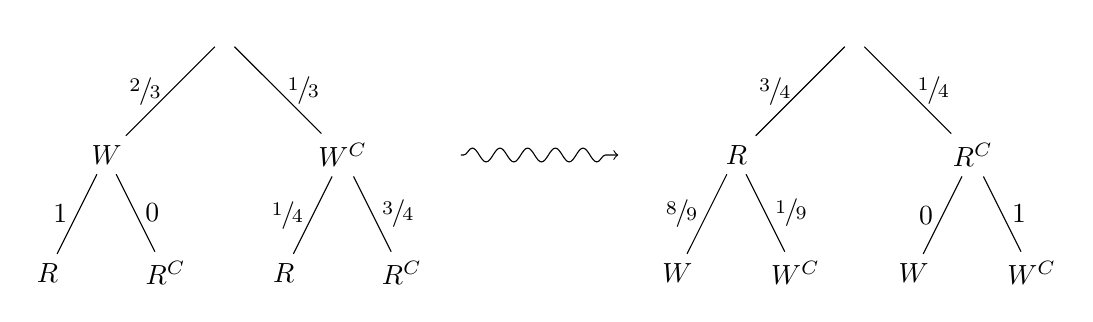
\begin{tikzpicture}[level distance=1.5cm,
		level 1/.style={sibling distance=3cm},
		level 2/.style={sibling distance=1.5cm},
		decoration = {snake, pre length=1pt, post length=1pt}]
		\node at (0,0) {}
		child {node {$W$}
			child {node {$R$} edge from parent node[left]  {$1$}}
			child {node {$R^C$} edge from parent node[right]  {$0$}}
			edge from parent
			node[left]  {$\sfrac{2}{3}$}
		}
		child {node {$W^C$}
			child {node {$R$} edge from parent node[left]  {$\sfrac{1}{4}$}}
			child {node {$R^C$} edge from parent node[right]  {$\sfrac{3}{4}$}}
			edge from parent
			node[right]  {$\sfrac{1}{3}$}
		};
		\draw[->,decorate] (3,-1.5) -- (5,-1.5);
		\node at (8,0) {}
		child {node {$R$}
			child {node {$W$} edge from parent node[left]  {$\sfrac{8}{9}$}}
			child {node {$W^C$} edge from parent node[right]  {$\sfrac{1}{9}$}}
			edge from parent
			node[left]  {$\sfrac{3}{4}$}
		}
		child {node {$R^C$}
			child {node {$W$} edge from parent node[left]  {$0$}}
			child {node {$W^C$} edge from parent node[right]  {$1$}}
			edge from parent
			node[right]  {$\sfrac{1}{4}$}
		};
	\end{tikzpicture}
	
\end{document}